% @Author: Sol W Courtney
% @Date:   2018-03-19 01:36:37
% @Last Modified by:   Sol W. Courtney
% @Last Modified time: 2018-03-19 16:23:11
%% --------------------------------------------------------------------------
%% DOCUMENT CLASS
%% --------------------------------------------------------------------------
\documentclass[11pt,a4paper,fleqn,notitlepage,oneside]{article}
	%\setlength{\cftsectionindent}{3em}
	%\setlength{\cftsubsectionindent}{4em}

%% --------------------------------------------------------------------------
%% PACKAGES
%% --------------------------------------------------------------------------
\usepackage[letterpaper, margin=1.0in]{geometry}
\usepackage[margin=2.5cm]{caption}
\usepackage{glossaries}
\usepackage{booktabs}
\usepackage{graphicx}
\usepackage{float}

%% --------------------------------------------------------------------------
%% SETTINGS
%% --------------------------------------------------------------------------
%\usefont{enc}{family}{series}{shape}
\pagenumbering{arabic}
    % arabic: arabic numerals
    % roman: lowercase roman numerals
    % Roman: uppercase roman numerals
    % alph: lowercase letters
    % Alph: uppercase letters 
\DeclareGraphicsExtensions{["png"]}
\graphicspath{{/home/sol/Github/skysearcher/data/plots/}}
\makeglossaries

%% --------------------------------------------------------------------------
%% GLOSSARY
%% --------------------------------------------------------------------------
% \newglossaryentry{duck}{
% 	name=duck,
% 	description={a waterbird with webbed feet}
% 	}
% 
% \newglossaryentry{parrot}{
% 	name=parrot, 
% 	description={mainly tropical bird with bright plumage}
% 	}

%% --------------------------------------------------------------------------
%% BEGIN DOCUMENT
%% --------------------------------------------------------------------------
\begin{document}

	%% ----------------------------------------------------------------------
	%% TITLE
	%% ----------------------------------------------------------------------
	\title{Defining WFIRST Survey Parameters: \\ Computational Methods}
	\author{Sol W. Courtney, Kathryn V. Johnston \& Robyn E. Sanderson \\ Columbia University Dept. Astronomy and Astrophysics}
	\date{\today}
	\maketitle
	
	%% ----------------------------------------------------------------------
	%% ABSTRACT
	%% ----------------------------------------------------------------------
	\begin{abstract}
		This document summarizes a first look at the possible parameters of a WFIRST survey of stellar halos around the 100 most luminous galaxies within 10Mpc of us. 
		There are broadly three aims of such surveys: (i) to look at the global properties of the halos (e.g. radial profile and total content); (ii) to find structures that are signatures of recent accretion events in order to examine broad properties and variety in accretion histories (including luminosity functions, rates and orbits); (iii) to find features at widest possible separations for subsequent spectroscopic follow up in order to place potential constraints.
		For all of the above purposes, the halos should be observed to the greatest radial extent possible.
		The extent to which this is possible or interesting will depend on expected densities of the stellar halos as well as contamination by background galaxies at faint magnitudes.
		The study “observes" the Bullock/Johnston stellar halo models as a guide for expectations (could be subsequently replaced with other models - e.g. FIRE).
	\end{abstract}

	%% ----------------------------------------------------------------------
	%% MAIN TEXT
	%% ----------------------------------------------------------------------
	%% 1 	\section{section}
	%% 2 	\subsection{subsection}
	%% 3 	\subsubsection{subsubsection}
	%% 4 	\paragraph{paragraph}
	%% 5 	\subparagraph{subparagraph}
	%% ----------------------------------------------------------------------
	%% SECTION #1 - The 100 Brightest Targets
	%% ----------------------------------------------------------------------
	\section[Observation Targets]{The 100 Brightest Targets} % (fold)
		\label{sec:the_100_brightest_targets}

		\subsection[NEARGALCAT]{Karachentsev's Catalog NEARGALCAT} % (fold)
			\label{sub:karachentsev_catalog_neargalcat}
			The Karachentsev\cite{2013AJ....145..101K} updated nearby galaxy catalog represents the nearest 869 galaxies.
			We are interested in observing those galaxies which are at least as luminous as the MilkyWay and therefore roughly equivalent in mass.
			Our goal is to sensibly select $100$\ targets from Karachentsev's original $869$\ galaxies.
			These target galaxies will serve as the underling layout for our simulated survey.

			\begin{table}[H]\centering
				\label{tab:karachentsev_catalog_neargalcat}
					\begin{tabular}{||c|cccc||}
						\hline 
						Unit & min & mean & max & std \\
						\midrule[1.5pt]
						$Distance\ (Mpc)$ & 0.02 & 6.98 & 26.2 & 4.19 \\
						$Abs_{B}mag$ & -21.8 & -13.83 & 0.0 & 3.42 \\
						\hline
					\end{tabular}
				\caption{
					Here we see the stats of the Karachentsev\cite{2013AJ....145..101K} catalog without the MilkyWay.
					$868$\ galaxies included.
					}
			\end{table}
		% subsection karachentsev_catalog_neargalcat (end)

		\subsubsection{Our Targets} % (fold)
			\label{ssub:our_targets}
			After sorting the list by distance we then select those galaxies which have an estimated distance of less than $10\ Mpc$.
			We then take the $100$\ most luminous of these targets as our $100$\ prospective targets.
			After selecting the targets, we calculate the minimum intrinsic brightness a star would need to be $M_{ab}Limit$\ in order to be perceptible at each target's estimated distance with the following.
			\[
			M_{ab}Limit = m^{filter}_{t_{exp}}limit - 5 * log_{10}(Distance*10^{6}\ Mpc/10pc)\ 
			\]
			\begin{table}[H]\centering
				\label{tab:our_targets}
					\begin{tabular}{||c|cccccc||}
						\hline 
						$Filter$ & Z087 & Y106 & J129 & H158 & F184 & W149\\
						\midrule[1.5pt]
						$1000\ second\ (m^{filter}_{1000sec}limit) $ & 27.15 & 27.13 & 27.14 & 27.12 & 26.15 & 27.67\\
						$2000\ second\ (m^{filter}_{2000sec}limit) $ & 27.9 & 27.88 & 27.89 & 27.87 & 26.9 & 28.42\\
						$t_{exp}$\ for $\sigma_{read}=\sigma_{sky}\ (seconds)$ & 200 & 190 & 180 & 180 & 240 & 90\\
					\hline
					\end{tabular}
				\caption{
					Here we see the WFIRST filter $1000$\ and $2000$\ second exposure imaging depths for each filter and $t_{exp}$\ for $\sigma_{read}=\sigma_{sky}\ (seconds)$
					}
			\end{table}

			From here onward we have selected the WFIRST H158 filter which has apparent magnitude limit of $27.87$\ when $t_{exp}=2000\ seconds$.
			The following table shows the $100$\ selected targets stats including the $M_{ab}Limit$\ for the target's distance as calculated with filter H158 for both $t_{exp}=1000\ seconds$\ and $t_{exp}=2000\ seconds$.
			$M_{ab}Limit$\ represents the estimated minimum intrinsic brightness a star needs to be precipitable.

			\begin{table}[H]\centering
				\label{tab:target_galaxies}
				\begin{tabular}{||c|cccc||}
					\hline 
					Unit & min & mean & max & std \\
					\midrule[1.5pt]
					$Distance\ (Mpc)$ & 0.82 & 4.54 & 7.2 & 1.5 \\
					$Abs_{B}mag$ & -21.3 & -17.39 & -15.1 & 1.64 \\
					$1000\ seconds\ M_{ab}Limit$ & -3.137 & -1.99 & 1.581 & 0.87 \\
					$2000\ seconds\ M_{ab}Limit$ & -1.414 & 0.26 & 3.304 & 0.87 \\
					\hline
				\end{tabular}
				\caption{
					Here we see the stats of our $100$\ most luminous target galaxies.
					$M_{ab}Limit$\ represents the minimum intrinsic brightness a star would need be if it is to be precipitable at the targets' estimated distance assuming filter H158 for both 1000 and 2000 second exposure times.
					}
			\end{table}
		% subsubsection our_targets (end)
	% section the_100_brightest_targets (end)

	\section[Observation Time]{Time Constraints} % (fold)
		\label{sec:time_constraints}
		The total required time for a survey seems to depend on 4 main factors.
		Fist there is the number of intended targets $(100)$.
		Second there is the extent of each halo intended to be photographed $(radial\ seperation\ Kpc)$.

		Third there is the estimated distance $(Mpc)$\ to each target and therefore the number of full fields of view $(N_{FoV})$.
		Fourth is the intended exposure time $(t_{exp})$\ for each $FoV$.
		Additionally there is the $slew/settle\ time$\ and the required time for target to target positioning.

		Putting this all together we can see that if $t_{exp}=2000\ seconds$\ one could tile/mosaic each of the 100 targets to a radial extent of 100 Kpc $(200\ Kpc\ box)$\ in approximately 2055 hours.
		Additionally there will be about 100 to 150 hours of movement.
		For a 200 Kpc box $(100\ Kpc\ seperation)$\ around each target there are in total approximately 3700 full WFIRST FoVs.
		Roughly 1241 square degrees in total, just about 3\% of the sky.

		\subsection{Total and Cumulative Time} % (fold)
			\label{sub:total_and_cumulative_time}

			Bellow is figure 1 showing the total $(in\ blue)$\ and cumulative $(in\ red)$\ amounts of both area $(on\ top)$\ and time $(on\ bottom)$\ associated with exposing a 200 Kpc box $(100\ Kpc\ seperation)$\ around each of our 100 proposed targets.
			The x-axis of both plots represents the distance to target, ranging from 0 to 8 $Mpc$.
			\begin{figure}[H]\centering
				\label{fig:all_targets}
				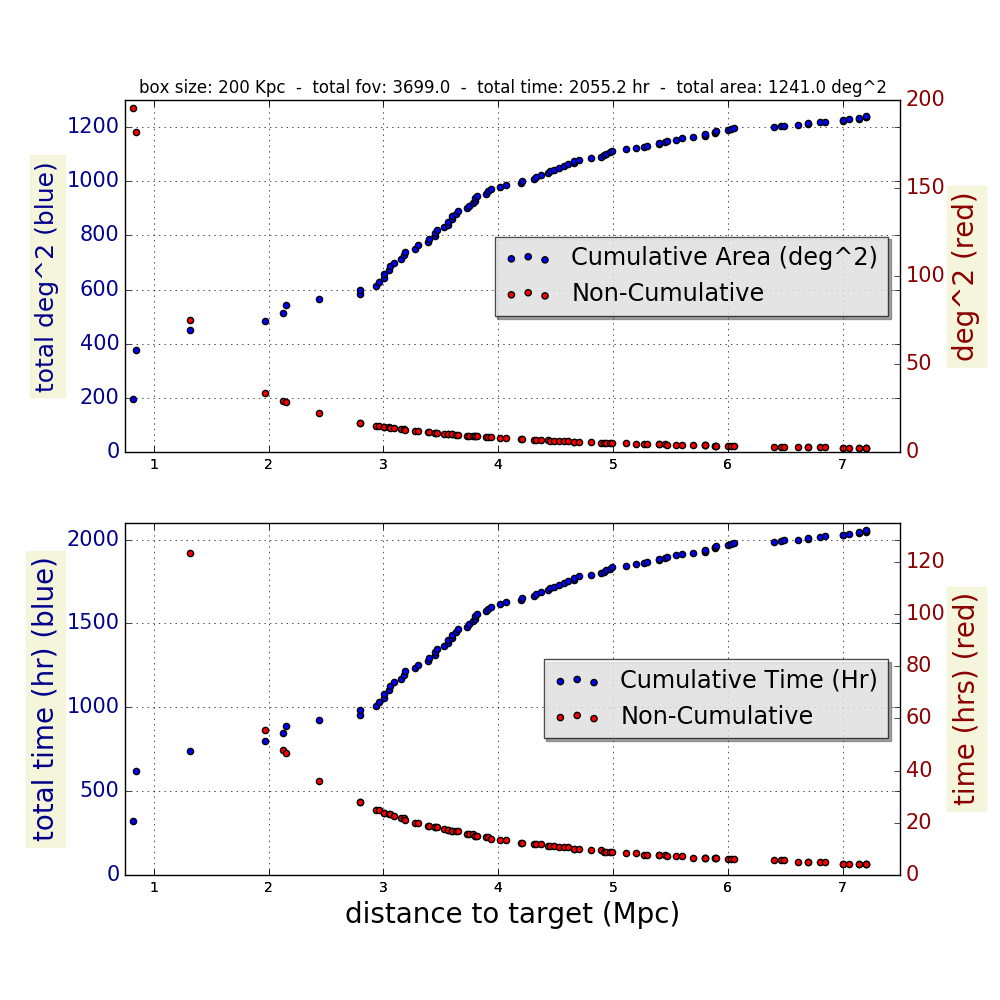
\includegraphics[width=0.85\textwidth]{all_targets.png}
				\caption{
					The top plot shows the the individual $(in\ red)$\ and cumulative $(in\ blue)$\ area $(deg^{2})$ covered by all 100 proposed target galaxies each having a 200 Kpc box $(radial\ seperation\ of\ 100\ Kpc)$.
					The bottom plot shows both the number of hours required for each target $(in\ red)$\ and the associated cumulative time $(in\ blue)$\ assuming a 2000 second exposure time.
				}
			\end{figure}	
		% subsection total_and_cumulative_time (end)
	% section time_constraints (end)


	%% ----------------------------------------------------------------------
	%% BIBLIOGRAPHY
	%% ----------------------------------------------------------------------
	\bibliography{mylib}{}
	\bibliographystyle{plain}

%% --------------------------------------------------------------------------
%% END DOCUMENT
%% --------------------------------------------------------------------------
\end{document}